\begin{document}
The selling price of the device can be seen below in Table \ref{fig:tablecost}.
\begin{figure}[H]
	\centering
	\caption{Cost Analysis Table}
	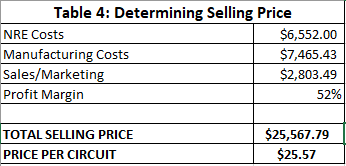
\includegraphics[width=0.7\linewidth]{tablecost}
	\label{fig:tablecost}
\end{figure}

While selling at a 52 \% profit margin the final price is a little less than \$26. This provides a competitive edge compared to similar products already on the market. It should be noted that users of the device will be expected to provide the batteries in order to power the device. Batteries were not included in the final cost in order to keep the price low for the consumer. It is assumed that for military applications propietary DoD power supplies will be used. The component value breakdown as well as non renewable engineering cost breakdown can be found in the appendix.

\end{document}